%%%%%%%%%%%%%%%%%%%%%%%%%%%%%%%%%%%%%%%%%%%%%%%%%%%%%%%%%%%%%%%%%%%%%%%%%%

%%%%%                           Conclusion Géné                     %%%%%%
%%%%%%%%%%%%%%%%%%%%%%%%%%%%%%%%%%%%%%%%%%%%%%%%%%%%%%%%%%%%%%%%%%%%%%%%%%

\phantomsection 
\addcontentsline{toc}{chapter}{General conclusion} \mtcaddchapter
\addtocontents{toc}{\protect\addvspace{10pt}}

\vspace*{-1cm}
\begin{flushright}
\section*{\fontsize{20pt}{20pt}\selectfont\textnormal{General conclusion}}
\end{flushright}
\vspace{2cm}

\lhead[\fancyplain{}{General conclusion}]
      {\fancyplain{}{}}
\chead[\fancyplain{}{}]
      {\fancyplain{}{}}
\rhead[\fancyplain{}{}] 
      {\fancyplain{}{General conclusion}}
\lfoot[\fancyplain{}{}]
      {\fancyplain{}{}}
\cfoot[\fancyplain{}{\thepage}]
      {\fancyplain{}{\thepage}}
\rfoot[\fancyplain{}{}]
     {\fancyplain{}{\scriptsize}}

%%%%%%%%%%%%%%%%%%%%%%%%%%%%%%%%%%%%%%%%%%%%%%%%%%%%%%%%%%%%%%%%%%%%%%%%%%
%%%%%                      Start part here                          %%%%%%
%%%%%%%%%%%%%%%%%%%%%%%%%%%%%%%%%%%%%%%%%%%%%%%%%%%%%%%%%%%%%%%%%%%%%%%%%%

\lettrine[lines=1]{C}{ }onclusion here.

The program also led to a collaboration with the CAMERA center (Center for the Analysis of Motion, Entertainment Research and Applications) of the University of Bath, to discussions with the Medical institute of University of Montreal, and to an in-person meeting with Matthew O'Neill from the Midwestern university. It has also been cited and reused in the field of 3D animation \cite{Barreto2022}, and quoted by the Stanford University, which later developed their own 3D markerless motion analysis solution \cite{Uhlrich2022}.

did a few experiments with balancing, dancing, and swimming, throwing

Target audience: sports scientists, not experts in computer vision, need for on-field analysis. GUI would help (CAMERA)
Would need more work to be usable in medical field. Can be used for 3D animation (Blender add-on)


\subsection{Issues related to OpenPose}

it could be interesting to build a new dataset, with more accurate labelling, more keypoints, trained on specific sports poses.

One way to solve this is enhancing the OpenPose dataset, by augmenting it with larger rotations so that upside-down poses are recognized, or by training it on specific sports poses. One risk of this approach is that the model may perform better on specific extreme poses, but worse on standard ones \cite{Kitamura2022}. 

Another approach, which could solve altogether the offsets in labeling, the dearth of keypoints, and the lack of accuracy on sports poses, could be to train on a whole new dataset. Note that this dataset should not base its labeling on marker positions, which could be interpreted as visual cues, that are not available in real sports situations. However, this condition is not sufficient: the dataset should also be large and diverse enough, represent a wide variety of body types and of sports movements \cite{Seethapathi2019}, and include images with motion blur such as found in sports videos. One way to do it is to build a synthetic dataset. For example, a mass of c3D motion files could be gathered from various sports, and be used to fit an SMPL+H mesh \cite{Pavlakos2019} with AMASS \cite{Mahmood2019}. These data could be augmented with already existing datasets for daily life activities, such as Agora \cite{Patel2021}. Then, it would be possible to take advantage of the fact that the topology of an SMPL mesh is constant, and assume that only labelling the first frame of any given sequence should be sufficient: label positions should be consistently propagated to the next frames. At this stage, one could place as many virtual markers as needed, for a precise evaluation of any movement and pose. However, only an expert should perform this task, and make sure that markers are correctly positioned: crowd-sourcing this task, like it is done for more basic image classification and segmentation with ImageNet \cite{Deng2009}, has been proved to lead to systematic offset errors \cite{Needham2021b}. Finally, random clothing, background, and light could be added (see \cite{Wood2021,Bolanos2021} for a detailed workflow), as well as variations in SMPL shape parameters. The scene would be filmed with numerous virtual cameras, in order to gather a large amount of diverse perspectives, and virtual markers would be automatically projected on the camera planes. This would result in an extensive sports dataset, created with minimal labelling work, on a potentially infinite amount of views. Nevertheless, before training the network, one should make sure that the generated data is as diverse as the real world, by using one of the metrics proposed by \cite{Borji2019, Borji2022}. Additionally, keypoint positions need to be precise enough: SMPL shape vertices can sometimes be more than 5 cm apart, which could cause imprecision errors similar to skin artifacts. Besides, instead of constraining pose estimation results with a physically consistent skeletal model, it would be interesting to develop a physics-informed pose estimation model \cite{Raissi2019}, which would offer the opportunity of embedding the kinematics priors as early as possible in the learning process.


SHAPE?

CALIBRATION / AUTO-CALIBRATION

MULTIPERSON

\subsection{inverse kinematics}
True to all constrained models, as opposed to 6DOF approaches: only applicable with population close to the norm: limb missing, pathological joint, not okay


GUI

Bath, MPP2SOS, Maya-Mocap (Blender MoCapViz)


\begin{figure}[hbtp]
      \centering
      \def\svgwidth{1\columnwidth}
      \fontsize{10pt}{10pt}\selectfont
      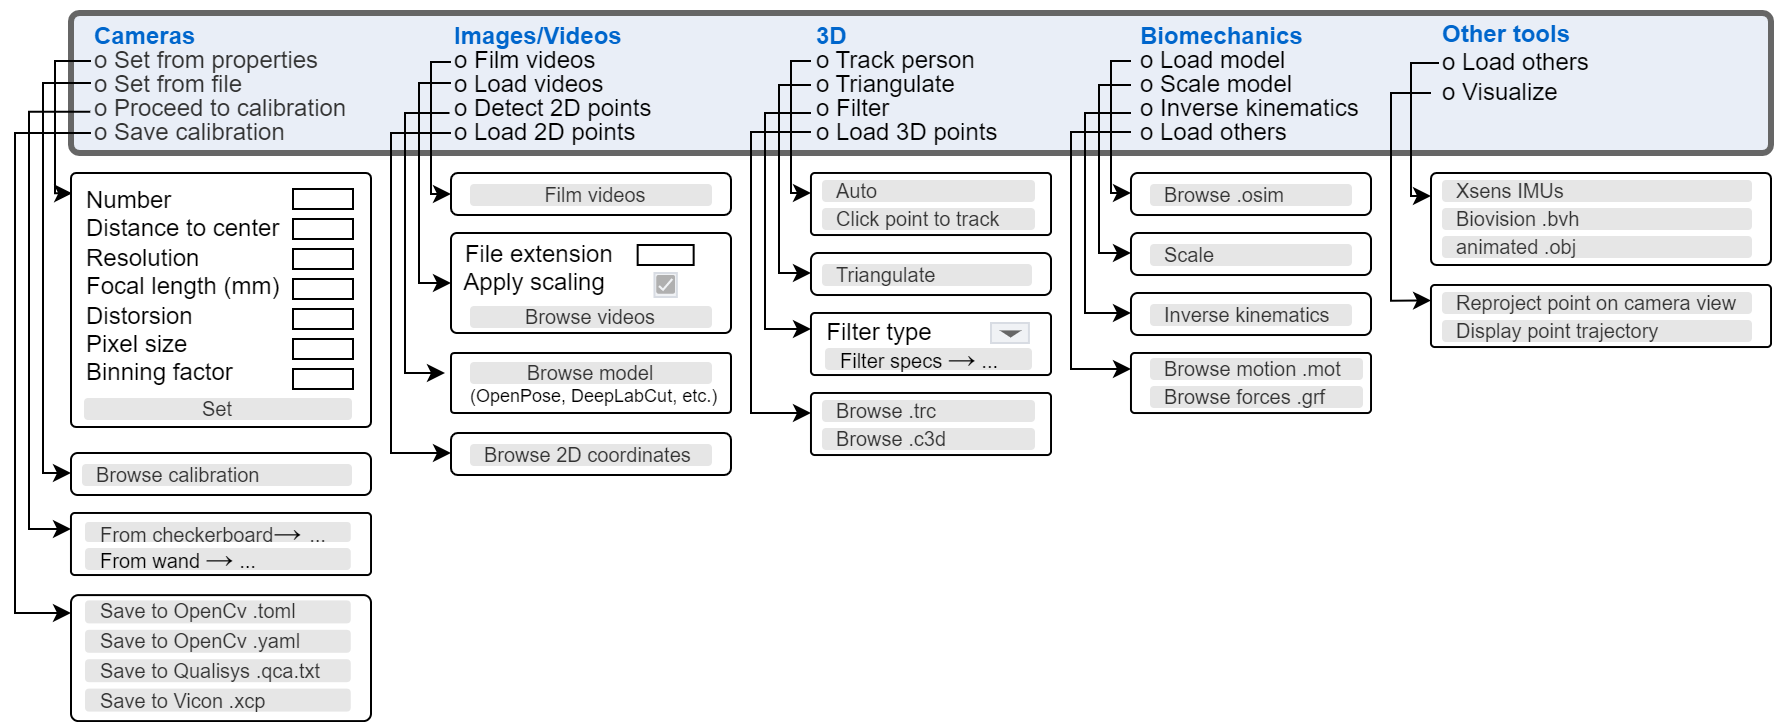
\includegraphics[width=\linewidth]{"../Chap3/Figures/Fig_MayaMocap3.png"}
      \caption{The organigram of Blender MoCapViz planned abilities.}
      \label{fig_blendermocap}
\end{figure}


% ajouter video de use on your own data
splashes, occlusions, distance, etc